

In this section we provide normal forms for the single-sorted one-step logics $\ofo$, $\ofoe$ and $\ofoei$. These normal forms will be pivotal to characterize the different fragments of these logics, in later sections.

\subsubsection{Normal form for $\ofo$}

We start by stating a normal form for one-step first-order logic without equality. A formula in \emph{basic form} gives a complete description of the types that are satisfied in a one-step model.

\index{form, basic!$\ofo$}
\index{$\dbnfofo{\Sigma}$}
\begin{definition}\label{def:bfofo}%[Basic form for \ofo]
A formula $\varphi \in \ofo(A)$ is in \emph{basic form} if $\varphi = \bigvee \dbnfofo{\Sigma}$
where each disjunct is of the form
\[
%\dbnfofo{\Sigma}{\Pi} = \bigwedge_{S\in\Sigma} \exists x. \tau_S(x) \land \forall x. \bigvee_{S\in\Pi} \tau_S(x)
\dbnfofo{\Sigma} = \bigwedge_{S\in\Sigma} \exists x. \tau_S(x) \land \forall x. \bigvee_{S\in\Sigma} \tau_S(x)
\]
%for some sets of types $\Sigma \subseteq \Pi \subseteq \wp A$ (observe the first $\subseteq$!).
for some set of types $\Sigma\subseteq \wp A$.
\end{definition}

It is easy to prove, using Ehrenfeucht-Fra\"iss\'e games, that every formula of first-order logic without equality over a unary signature (i.e., $\ofo$) is equivalent to a formula in basic form. Proof sketches can be found in~\cite[Lemma 16.23]{Graedel2002} and~\cite[Proposition 4.14]{Venema2014}. We omit a full proof because it is very similar to the following more complex cases.

\begin{fact}\label{fact:ofonormalform}
Every formula of $\ofo(A)$ is equivalent to a formula in basic form.
\end{fact}

%%%%
\subsubsection{Normal form for $\ofoe$}

When considering a normal form for $\ofoe$, the fact that we can `count types' using equality yields a more involved basic form.

\index{form, basic!$\ofoe$}
\index{$\dbnfofoe{\vlist{T}}{\Pi}$}
\begin{definition}%[Basic form for \ofoe]
We say that a formula $\varphi \in \ofoe(A)$ is in \emph{basic form} if $\varphi = \bigvee \dbnfofoe{\vlist{T}}{\Pi}$ where each disjunct is of the form
%
\begin{equation*}%\label{eq:normalformofoe}
\dbnfofoe{\vlist{T}}{\Pi} = \exists \vlist{x}.\big(\arediff{\vlist{x}} \land \bigwedge_i \tau_{T_i}(x_i) \land \forall z.(\arediff{\vlist{x},z} \lthen \bigvee_{S\in \Pi} \tau_S(z))\big)
\end{equation*}
%
such that $\vlist{T} \in \wp(A)^k$ for some $k$ and $\Pi \subseteq \vlist{T}$.  The predicate $\arediff{\vlist{y}}$, stating that the elements $\vlist{y}$ are distinct, is defined as $\arediff{y_1,\dots,y_n} := \bigwedge_{1\leq m < m^{\prime} \leq n} (y_m \not\approx y_{m^{\prime}})$.
\end{definition}

We prove that every formula of monadic first-order logic with equality (i.e., $\ofoe$) is equivalent to a formula in basic form. This result seems to be folklore, however, we provide a detailed proof because some of its ingredients will be used later, when we give a normal form for $\ofoei$. We start by defining the following relation between one-step models.

% \index{$\sim^=_k$}
\begin{definition}
	Let $\osmodel$ and $\osmodel'$ be one-step models. For every $k \in \nat$, the relation $\osmodel \sim^=_k \osmodel'$ is defined as
\begin{eqnarray*}
	\osmodel \sim^=_k \osmodel' & \Longleftrightarrow & \forall S\subseteq A \ \big(
	   |S|_\osmodel = |S|_{\osmodel'} < k \\
	&& \qquad\qquad \text{or } |S|_\osmodel,|S|_{\osmodel'} \geq k \big)
\end{eqnarray*}
\end{definition}

Intuitively, two models are related by $\sim^=_k$ when their type information coincides `modulo~$k$'. Later we will prove that this is the same as saying that they cannot be distinguished by a formula of $\ofoe$ with quantifier rank lower or equal to $k$. For the moment, we prove the following properties of $\sim^=_k$.

\begin{proposition}\label{props:eqrelofoe} The following hold:
	\begin{enumerate}[(i)]
		\itemsep 0 pt
		\item $\sim^=_k$ is an equivalence relation,
		\item $\sim^=_k$ has finite index,
		\item Every $E \in \umods/{\sim^=_k}$ is characterized by a formula $\varphi^=_E \in \ofoe(A)$ with $qr(\varphi^=_E) = k$.
	\end{enumerate}
\end{proposition}
\begin{proof}
	We only prove the last point. Let $E \in \umods/{\sim^=_k}$ and let $\osmodel \in E$ be a representative. Call $S_1,\dots,S_n \subseteq A$ to the types such that $|S_i|_\osmodel = n_i < k$ and $S'_1,\dots,S'_m \subseteq A$ to those satisfying $|S'_i|_\osmodel \geq k$. Now define
	%
	\begin{align*}
	\varphi^=_E := & \bigwedge_{i\leq n} \big(\exists x_1,\dots,x_{n_i}.\arediff{x_1,\dots,x_{n_i}} \ \land \\
		& \qquad\bigwedge_{j\leq n_i} \tau_{S_i}(x_j) \land \forall z. \arediff{x_1,\dots,x_{n_i},z} \lthen \lnot\tau_{S_i}(z)\big)\ \land \\
	    & \bigwedge_{i\leq m} \big(\exists x_1,\dots,x_k.\arediff{x_1,\dots,x_k} \land \bigwedge_{j\leq k} \tau_{S'_i}(x_j) \big)
	            %& \bigwedge_{i\leq m} \big(\forall x_1,\dots,x_{k-1}.\exists x_k.\arediff{x_1,\dots,x_{k}} \land \bigwedge_{j\leq k} \tau_{S'_i}(x_j) \big)
	\end{align*}
	%
	First note that the union of all the $S_i$ and $S'_i$ yields all the possible $A$-types, and that if a type is not realized at all, then it will correspond to some $S_j$ with $n_j = 0$. It is easy to see that $qr(\varphi^=_E) = k$ and that $\osmodel' \models \varphi^=_E$ iff $\osmodel' \in E$. Observe that $\varphi^=_E$ gives a specification of $E$ ``type by type''.
\end{proof}

Next we recall a (standard) notion of Ehrenfeucht-Fra\"iss\'e game for $\ofoe$ which will be used to establish the connection between ${\sim^=_k}$ and $\equiv_k^\foe$.

% \index{$\efgame^=_k(\osmodel_0,\osmodel_1)$}
\begin{definition}
	Let $\osmodel_0 = (D_0,\val_0)$ and $\osmodel_1 = (D_1,\val_1)$ be one-step models. We define the game $\efgame^=_k(\osmodel_0,\osmodel_1)$ between \abelard and \eloise. If $\osmodel_i$ is one of the models we use $\osmodel_{-i}$ to denote the other model. A position in this game is a pair of sequences $\vlist{s_0} \in D_0^n$ and $\vlist{s_1} \in D_1^n$ with $n \leq k$. The game consists of $k$ rounds where in round $n+1$ the following steps are made
	%
	\begin{enumerate}[1.]
		\itemsep 0 pt
		\parsep 0 pt
		\item \abelard chooses an element $d_i$ in one of the $\osmodel_i$,
		\item \eloise responds with an element $d_{-i}$ in the model $\osmodel_{-i}$.
		\item Let $\vlist{s_i} \in D_i^n$ be the sequences of elements chosen up to round $n$, they are extended to ${\vlist{s_i}' := \vlist{s_i}\cdot d_i}$. Player \eloise survives the round iff she does not get stuck and the function $f_{n+1}: \vlist{s_0}' \mapsto \vlist{s_1}'$ is a partial isomorphism of one-step models.
	\end{enumerate}
	%
	Player \eloise wins iff she can survive all $k$ rounds.
	%
	%At the end of the game we have a sequence of $k$ pairs $(d_0^i,d_1^i)$. The match is won by \eloise iff she never gets stuck and the function $f: d_0^i \mapsto d_1^i$ is a partial isomorphism of one-step models, that is, $f$ is bijective and $d \in \val_0(a) \Leftrightarrow f(d) \in \val_1(a)$ for all $a\in A$.
	%
	Given $n\leq k$ and $\vlist{s_i} \in D_i^n$ such that $f_n:\vlist{s_0}\mapsto\vlist{s_1}$ is a partial isomorphism, we use $\efgame_{k}^=(\osmodel_0,\osmodel_1)@(\vlist{s_0},\vlist{s_1})$ to denote the (initialized) game where $n$ moves have been played and $k-n$ moves are left to be played.
\end{definition}

\begin{lemma}\label{lem:connofoe}
	The following are equivalent
	\begin{enumerate}
		\itemsep 0 pt
		\item\label{lem:connofoe:i} $\osmodel_0 \equiv_k^\foe \osmodel_1$,
		\item\label{lem:connofoe:ii} $\osmodel_0 \sim_k^= \osmodel_1$,
		\item\label{lem:connofoe:iii} \eloise has a winning strategy in $\efgame_k^=(\osmodel_0,\osmodel_1)$.
	\end{enumerate}
\end{lemma}
\begin{proof}
	Step~(\ref{lem:connofoe:i}) to~(\ref{lem:connofoe:ii}) is direct by Proposition~\ref{props:eqrelofoe}. For~(\ref{lem:connofoe:ii}) to~(\ref{lem:connofoe:iii}) we give a winning strategy for \eloise in $\efgame_k^=(\osmodel_0,\osmodel_1)$. We do it by showing the following claim
	%
	\begin{claimfirst}
	Let $\osmodel_0 \sim_k^= \osmodel_1$ and $\vlist{s_i} \in D_i^n$ be such that $n<k$ and $f_n:\vlist{s_0}\mapsto\vlist{s_1}$ is a partial isomorphism; then \eloise can survive one more round in $\efgame_{k}^=(\osmodel_0,\osmodel_1)@(\vlist{s_0},\vlist{s_1})$.
	\end{claimfirst}
	%
	\begin{pfclaim}
		Let \abelard pick $d_i\in D_i$ such that the type of $d_i$ is $T \subseteq A$. If $d_i$ had already been played then \eloise picks the same element as before and $f_{n+1} = f_n$. If $d_i$ is new and $|T|_{\osmodel_i} \geq k$ then, as at most $n<k$ elements have been played, there is always some new $d_{-i} \in D_{-i}$ that \eloise can choose that matches $d_i$. If $|T|_{\osmodel_i} = m < k$ then we know that $|T|_{\osmodel_{-i}} = m$. Therefore, as $d_i$ is new and $f_n$ is injective, there must be a $d_{-i} \in D_{-i}$ that \eloise can choose. %This shows how to extend the partial isomorphism given by the $(k-1)$-round game to a partial isomorphism for the $k$-round game.
	\end{pfclaim}
	
	Step~(\ref{lem:connofoe:iii}) to~(\ref{lem:connofoe:i}) is a standard result~\cite[Corollary 2.2.9]{fmt} which we prove anyway because we will need to extend it later. We prove the following loaded statement.
	\begin{claim}
		Let $\vlist{s_i} \in D_i^n$ and $\varphi(z_1,\dots,z_n) \in \ofoe(A)$ be such that $qr(\varphi) \leq k-n$. If \eloise has a winning strategy in the game $\efgame_k^=(\osmodel_0,\osmodel_1)@(\vlist{s_0},\vlist{s_1})$ then $\osmodel_0 \models \varphi(\vlist{s_0})$ iff $\osmodel_1 \models \varphi(\vlist{s_1})$.
	\end{claim}
	%
	\begin{pfclaim}
		If $\varphi$ is atomic the claim holds because of $f_n:\vlist{s_0}\mapsto \vlist{s_1}$ being a partial isomorphism. Boolean cases are straightforward.
		%
		Let $\varphi(z_1,\dots,z_n) = \exists x. \psi(z_1,\dots,z_n,x)$ and suppose $\osmodel_0 \models \varphi(\vlist{s_0})$. Hence, there exists $d_0 \in D_0$ such that $\osmodel_0 \models \psi(\vlist{s_0},d_0)$.
		%
		By hypothesis we know that \eloise has a winning strategy for $\efgame_k^=(\osmodel_0,\osmodel_1)@(\vlist{s_0},\vlist{s_1})$. Therefore, if \abelard picks $d_0\in D_0$ she can respond with some $d_1\in D_1$ and has a winning strategy for $\efgame_{k}^=(\osmodel_0,\osmodel_1)@(\vlist{s_0}{\cdot}d_0,\vlist{s_1}{\cdot}d_1)$.
		%
		By induction hypothesis, because $qr(\psi) \leq k- (n+1)$, we have that $\osmodel_0 \models \psi(\vlist{s_0},d_0)$ iff $\osmodel_1 \models \psi(\vlist{s_1},d_1)$ and hence $\osmodel_1 \models \exists x.\psi(\vlist{s_1},x)$. The opposite direction is proved by a symmetric argument. %and the case where $\varphi$ is $\forall x. \psi(z_1,\dots,z_n,x)$ are very similar.
		\end{pfclaim}
		%
		Combining these claims finishes the proof of the lemma.
\end{proof}

\begin{theorem}\label{thm:bnfofoe}
Every $\psi \in \ofoe(A)$ is equivalent to a formula in basic form.
\end{theorem}
\begin{proof}
	Let $qr(\psi) = k$ and let $\ext{\psi}$ be the class of models satisfying $\psi$. As $\umods/{\equiv_k^\foe}$ is the same as $\umods/{\sim_k^=}$ by Lemma~\ref{lem:connofoe}, it is easy to see that $\psi$ is equivalent to $\bigvee \{ \varphi^=_E \mid E \in \ext{\psi}/{\sim_k^=} \}$. Now it only remains to see that each $\varphi^=_E$ is equivalent to $\dbnfofoe{\vlist{T}}{\Pi}$ for some $\Pi \subseteq \wp A$ and $T_i \subseteq A$.

	The crucial observation is that we will use $\vlist{T}$ and $\Pi$ to give a specification of the types ``element by element''. Let $\osmodel \in E$ be a representative. Call $S_1,\dots,S_n \subseteq A$ to the types such that $|S_i|_\osmodel = n_i < k$ and $S'_1,\dots,S'_m \subseteq A$ to those satisfying $|S'_i|_\osmodel \geq k$. The size of the sequence $\vlist{T}$ is defined to be $(\sum_{i=1}^n n_i) + k\times m$ where $\vlist{T}$ is contains exactly $n_i$ occurrences of type $S_i$ and $k$ occurrences of each $S'_j$. On the other hand $\Pi = \{S'_1,\dots,S'_m\}$. It is straightforward to check that $\varphi^=_E$ is equivalent to $\dbnfofoe{\vlist{T}}{\Pi}$, however, the quantifier rank of the latter is only bounded by $k\times 2^{|A|} + 1$.
\end{proof}

%%%%
\subsubsection{Normal form for $\ofoei$}

The logic $\ofoei$ extends $\ofoe$ with the capacity to tear apart finite and infinite sets of elements. This is reflected in the normal form for $\ofoei$ by adding extra constraints to the normal form of $\ofoe$.

\index{form, basic!$\ofoei$}
\index{$\dbnfofoei{\vlist{T}}{\Pi}{\Sigma}$}
\index{$\dbnfinf{\Sigma}$}
\begin{definition}\label{def:basicform_fofoei}
We say that a formula $\varphi \in \ofoei(A)$ is in \emph{basic form} if $\varphi = \bigvee \dbnfofoei{\vlist{T}}{\Pi}{\Sigma}$ where each disjunct is of the form
%
\[
\dbnfofoei{\vlist{T}}{\Pi}{\Sigma} = \dbnfofoe{\vlist{T}}{\Pi \cup \Sigma} \land \dbnfinf{\Sigma}
\]
where
\[
\dbnfinf{\Sigma} := \bigwedge_{S\in\Sigma} \qu y.\tau_S(y) \land \dqu y.\bigvee_{S\in\Sigma} \tau_S(y)
\]
%
for some set of types $\Pi,\Sigma \subseteq \wp A$ and each $T_i \subseteq A$.
\end{definition}

Intuitively, the formula $\dbnfinf{\Sigma}$ says that (1) for every type $S\in\Sigma$, there are infinitely many elements satisfying $S$ and (2) only finitely many elements do not satisfy any type in $\Sigma$.

A short argument reveals that, intuitively, every disjunct expresses that each one-step model satisfying it admits a partition of its domain in three parts:
\begin{enumerate}[(i)]
\itemsep 0 pt
\item distinct elements $t_1,\dots,t_n$ with type $T_1,\dots,T_n$,
\item finitely many elements whose types belong to $\Pi$, and
\item for each $S\in \Sigma$, infinitely many elements with type $S$.
\end{enumerate}

In the same way as before, we define a relation $\sim^\infty_k$ which refines $\sim^=_{k}$ by adding information about the (in-)finiteness of the types.

% \index{$\sim^\infty_k$}
\begin{definition}
	Let $\osmodel$ and $\osmodel'$ be one-step models. For every $k\in\nat$, the relation $\osmodel \sim^\infty_k \osmodel'$ is defined as follows:
\begin{eqnarray*}
	\osmodel \sim^\infty_0 \osmodel' & \Longleftrightarrow & \text{always}\\
	\osmodel \sim^\infty_{k+1} \osmodel' & \Longleftrightarrow & \osmodel \sim^=_{k+1} \osmodel' \text{ and }\\
	&& \forall S\subseteq A \ \big(
	|S|_\osmodel,|S|_{\osmodel'} < \omega \text{ or } |S|_\osmodel,|S|_{\osmodel'} \geq \omega \big)%\\
	%&& \qquad\qquad \text{or } |S|_\osmodel,|S|_{\osmodel'} \geq \omega \big)
\end{eqnarray*}
\end{definition}

\begin{proposition}\label{props:eqrelolque} The following hold:
	\begin{enumerate}[(i)]
		\itemsep 0 pt
		\item $\sim^\infty_k$ is an equivalence relation,
		\item $\sim^\infty_k$ has finite index,
		\item $\sim^\infty_k$ is a refinement of $\sim^=_k$,
		\item Every $E \in \umods/{\sim^\infty_k}$ is characterized by a formula $\varphi^\infty_E \in \ofoei(A)$ with $qr(\varphi) = k$.
	\end{enumerate}
\end{proposition}
\begin{proof}
	We only prove the last point, for $k>0$. Let $E \in \umods/{\sim^\infty_k}$ and let $\osmodel \in E$ be a representative of the class. Let $E' \in \umods/{\sim^=_k}$ be the equivalence class of $\osmodel$ with respect to $\sim^=_k$.
	%
	Let $S_1,\dots,S_n \subseteq A$ be all the types such that $|S_i|_\osmodel \geq \omega$. % and $S'_1,\dots,S'_m \subseteq A$ to those satisfying $|S'_i|_\osmodel < \omega$. Now define
	%
	\[
	\varphi^\infty_E := \varphi^=_{E'} \land
		% \bigwedge_{i\leq n} \qu x.\tau_{S_i}(x) \land \bigwedge_{i\leq m} \dqu x.\lnot\tau_{S'_i}(x) .
		\dbnfinf{\{S_1,\dots,S_n\}} .
	\]
	%
	It is not difficult to see that $qr(\varphi^\infty_E) = k$ and that $\osmodel' \models \varphi^\infty_E$ iff $\osmodel' \in E$. %Observe again, that $\varphi^\infty_E$ gives a specification of $E$ ``type by type''.
\end{proof}

Now we give a notion of Ehrenfeucht-Fra\"ss\'e game for $\ofoei$. In this case the game extends $\efgame^=_k$ with a move for $\qu$.

% \index{$\efgame^\infty_k(\osmodel_0,\osmodel_1)$}
\begin{definition}
	Let $\osmodel_0 = (D_0,\val_0)$ and $\osmodel_1 = (D_1,\val_1)$ be one-step models. We define the game $\efgame^\infty_k(\osmodel_0,\osmodel_1)$ between \abelard and \eloise. A position in this game is a pair of sequences $\vlist{s_0} \in D_0^n$ and $\vlist{s_1} \in D_1^n$ with $n \leq k$. The game consists of $k$ rounds, where in round $n+1$ the following steps are made. First \abelard chooses to perform one of the following types of moves:
	%
	\begin{enumerate}[(a)]
		\itemsep 0 pt
		\parsep 0 pt
		%
		\item Second-order move
		\begin{enumerate}[1.]
			\itemsep 0 pt
			\parsep 0 pt
			\item \abelard chooses an infinite set $X_i \subseteq D_i$,
			\item \eloise responds with an infinite set $X_{-i} \subseteq D_{-i}$,
			%\item {\color{red} This is probably not needed anymore (according to~\cite{Kolaitis199523}):} Given a fresh name $s \notin A$ the models are extended to $\osmodel_i = (M_i, \val_i[s \mapsto X_i])$,
			\item \abelard chooses an element $x_{-i} \in X_{-i}$,
			\item \eloise responds with an element $x_i \in X_i$.
		\end{enumerate}
		%
		\item First-order move
		\begin{enumerate}[1.]
			\itemsep 0 pt
			\parsep 0 pt
			\item \abelard chooses an element $d_i \in D_i$,
			\item \eloise responds with an element $d_{-i} \in D_{-i}$.
		\end{enumerate}
	\end{enumerate}
	%
	Let $\vlist{s_i} \in D_i^n$ be the sequences of elements chosen up to round $n$, they are extended to ${\vlist{s_i}' := \vlist{s_i}\cdot d_i}$. \eloise survives the round iff she does not get stuck and the function $f_{n+1}: \vlist{s_0}' \mapsto \vlist{s_1}'$ is a partial isomorphism of one-step models.
\end{definition}

This game can be seen as an adaptation of the Ehrenfeucht-Fra\"ss\'e game for monotone generalized quantifiers found in~\cite{Kolaitis199523} to the case of full monadic first-order logic. %see Def 3.2, 3.8 and Thm 3.9.

\begin{lemma}\label{lem:connolque}
	The following are equivalent:
	\begin{enumerate}
		\itemsep 0 pt
		\item\label{lem:connolque:i} $\osmodel_0 \equiv_k^{\foei} \osmodel_1$,
		\item\label{lem:connolque:ii} $\osmodel_0 \sim_k^\infty \osmodel_1$,
		\item\label{lem:connolque:iii} \eloise has a winning strategy in $\efgame_k^\infty(\osmodel_0,\osmodel_1)$.
	\end{enumerate}
\end{lemma}

%{\color{red} The $\equiv_k$ is probably not ok. For example, we have much more succinctness to count in WMSO: we can say ``there are $2n$ elements'' with a formula of quantifier rank $n+1$ using $\exists X. (\exists x_1\dots x_n. x_i\in X) \land (\exists x_1\dots x_n. x_i\notin X)$. Should it be $2^k$ somewhere?}

\begin{proof}
	Step~(\ref{lem:connolque:i}) to~(\ref{lem:connolque:ii}) is direct by Proposition~\ref{props:eqrelolque}. For~(\ref{lem:connolque:ii}) to~(\ref{lem:connolque:iii}) we show
	%
	\begin{claimfirst}
	Let $\osmodel_0 \sim_k^\infty \osmodel_1$ and $\vlist{s_i} \in D_i^n$ be such that $n<k$ and $f_n:\vlist{s_0}\mapsto\vlist{s_1}$ is a partial isomorphism; then \eloise can survive one more round in $\efgame_{k}^\infty(\osmodel_0,\osmodel_1)@(\vlist{s_0},\vlist{s_1})$.
	% Let $\osmodel_0 \sim_k^\infty \osmodel_1$, $n<k$ and $\vlist{r_n} \in D_0^n$, $\vlist{s_n} \in D_1^n$ be  such that $f_n:\vlist{r_n}\mapsto\vlist{s_n}$ is a partial isomorphism; then \eloise can survive one more round in $\efgame_{k}^\infty(\osmodel_0,\osmodel_1)@(\vlist{r_n},\vlist{s_n})$.
	\end{claimfirst}
	%
	\begin{pfclaim}
		We focus on the second-order moves because the first-order moves are the same as in the corresponding Claim of Lemma~\ref{lem:connofoe}. Let \abelard choose an infinite set $X_i \subseteq D_i$, we would like \eloise to choose a set $X_{-i} \subseteq D_{-i}$ such that the following conditions hold:
		%
		\begin{enumerate}[(a)]
			\parskip 0pt
			%
			\item\label{it:piso} %For $j\in\{0,1\}$ let $\vlist{r_j} := \vlist{s_j}\cap X_j$ be the restriction of $\vlist{s_j}$ to the elements of $X_j$. We want 
			The map $f_n$ is a well-defined partial isomorphism between the restricted one-step models $\osmodel_0{\rest}X_0$ and $\osmodel_1{\rest}X_1$,
			%
			\item\label{it:equiv}
			For every type $S$ we have that there is an element $d\in X_i$ of type $S$ which is \emph{not} connected by $f_n$ iff there is such an element in $X_{-i}$,
			% $\osmodel_0{\rest}X_0 \sim_{m+1}^= \osmodel_1{\rest}X_1$ where $m = |r_i|$. That is, for all $S \subseteq A$,
			% \begin{enumerate}[(i)]
			% 	\itemsep 0pt
			% 	\item if $|S|_{X_i} < m+1$ then $|S|_{X_{-i}} = |S|_{X_i}$,
			% 	\item if $|S|_{X_i} \geq m+1$ then $|S|_{X_{-i}} \geq m+1$,
			% 	%\item if $|S|_{X_i} \geq \omega$ then $|S|_{X_{-i}} \geq \omega$,
			% \end{enumerate}
			%
			\item\label{it:inf} $X_{-i}$ is infinite.
		\end{enumerate}
		%
		First we prove that such a set exists. % and then we will use it to prove the claim.
		%
		To satisfy item~\eqref{it:piso} she just needs to add to $X_{-i}$ the elements connected to $X_i$ by $f_n$; this is not a problem.

%		\begin{figure}
%			\centering
%			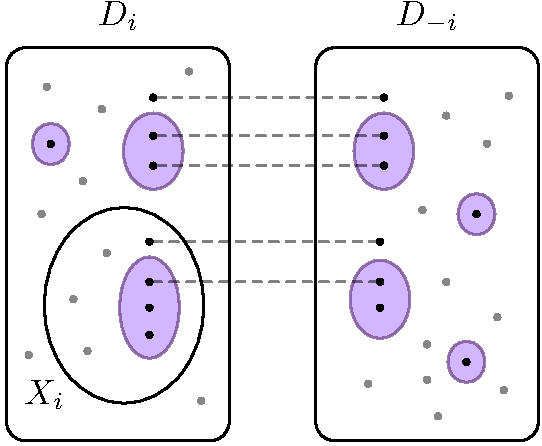
\includegraphics[scale=0.9]{chapter5/fig-efinf.pdf}
%			% \caption{$k=10, n=5, m=2, |S|_{X_i}=3$ and $|S|_{D_i}=|S|_{D_{-i}}=6$.}
%			\caption{Elements of type $S$ have coloured background.}
%			\label{fig:efinf}
%		\end{figure}

		For item~\eqref{it:equiv} we proceed as follows: for every type $S$ such that there is an element $d\in X_i$ of type $S$, we add a new element $d'\in D_{-i}$ of type $S$ to $X_{-i}$. To see that this is always possible, observe first that $\osmodel_0 \sim_k^\infty \osmodel_1$ implies $\osmodel_0 \sim_k^= \osmodel_1$. Using the properties of this relation, we divide in two cases:
		%
		\begin{itemize}
			\item If $|S|_{D_i} \geq k$ we know that $|S|_{D_{-i}} \geq k$ as well. From the elements of $D_{-i}$ of type $S$, at most $n<k$ are used by $f_n$. Hence, there is at least one $d'\in D_{-i}$ of type $S$ to choose from.
			%
			\item If $|S|_{D_i} < k$ we know that $|S|_{D_{i}} = |S|_{D_{-i}}$. From the elements of $D_{i}$ of type $S$, at most $|S|_{D_{i}}-1$ are used by $f_n$. The reason for the $-1$ is that we are assuming that we have just chosen a $d\in X_i$ which is not in $f_n$. Using that $|S|_{D_{i}} = |S|_{D_{-i}}$ and that $f_n$ is a partial isomorphism we can again conclude that there is at least one $d'\in D_{-i}$ of type $S$ to choose from.
		\end{itemize}
		%
		For item~\eqref{it:inf} observe that as $X_{i}$ is infinite but there are only finitely many types, there must be some $S$ such that $|S|_{X_i} \geq \omega$. It is then safe to add infinitely many elements for $S$ in $X_{-i}$ while considering point~\eqref{it:equiv}. Moreover, the existence of infinitely many elements satisfying $S$ in $D_{-i}$ is guaranteed by $\osmodel_0 \sim_k^\infty \osmodel_1$.

		Having shown that \eloise can choose a set $X_{-i}$ satisfying the above conditions, it is now clear that using point~\eqref{it:equiv} \eloise can survive the ``first-order part'' of the second-order move we were considering. This finishes the proof of the claim.
		% we continue the proof of the claim as follows: as $\osmodel_0{\rest}X_0 \sim_{m+1}^= \osmodel_1{\rest}X_1$ and $f':\vlist{r_0}\mapsto\vlist{r_1}$ is a partial isomorphism between them (with sequences of length $m$) then by the first claim of Lemma~\ref{lem:connofoe}, we know that \eloise can survive one round in $\efgame_{m+1}^=(\osmodel_0{\rest}X_0,\osmodel_1{\rest}X_1)@(\vlist{r_0},\vlist{r_1})$. In particular, she can survive the ``first-order part'' of the second-order move we were considering. This finishes the proof of the claim.
	\end{pfclaim}
	%
	Going back to the proof of Lemma~\ref{lem:connolque}, for step~(\ref{lem:connolque:iii}) to~(\ref{lem:connolque:i}) we prove the following.
	%
	\begin{claim}
		Let $\vlist{s_i} \in D_i^n$ and $\varphi(z_1,\dots,z_n) \in \ofoei(A)$ be such that $qr(\varphi) \leq k-n$. If \eloise has a winning strategy in $\efgame_k^\infty(\osmodel_0,\osmodel_1)@(\vlist{s_0},\vlist{s_1})$ then $\osmodel_0 \models \varphi(\vlist{s_0})$ iff $\osmodel_1 \models \varphi(\vlist{s_1})$.
	\end{claim}
	%
	\begin{pfclaim}
		All the cases involving operators of \ofoe are the same as in Lemma~\ref{lem:connofoe}. We prove the inductive case for the generalized quantifier. Let $\varphi(z_1,\dots,z_n)$ be of the form $\qu x.\psi(z_1,\dots,z_n,x)$ and let $\osmodel_0 \models \varphi(\vlist{s_0})$. Hence, there is an \emph{infinite} set $X_0 \subseteq D_0$ such that
		%
		\begin{equation}\label{eq:ind0ok}
		\osmodel_0 \models \psi(\vlist{s_0},x_0) \text{ if and only if } x_0\in X_0 .
		\end{equation}
		%
		By hypothesis we know that \eloise has a winning strategy for $\efgame_k^\infty(\osmodel_0,\osmodel_1)@(\vlist{s_0},\vlist{s_1})$. Therefore, if \abelard plays a second-order move by picking $X_0 \subseteq D_0$ she can respond with some infinite set $X_1 \subseteq D_1$. We claim that $\osmodel_1 \models \psi(\vlist{s_1},x_1)$ for every $x_1\in X_1$. First observe that if this holds then the set $X'_1 := \{ d_1 \in D_1 \mid \osmodel_1 \models \psi(\vlist{s_1},d_1)\}$ must be infinite, and hence $\osmodel_1 \models \qu x.\psi(\vlist{s_1},x)$.% and we are done.
		
		Assume, for a contradiction, that $\osmodel_1 \not\models \psi(\vlist{s_1},x'_1)$ for some $x'_1\in X_1$. Let \abelard play that $x'_1$ as the second part of his move. Then, as \eloise has a winning strategy, she will respond with some $x'_0 \in X_0$ such that she has a winning strategy for $\efgame_{k}^\infty(\osmodel_0,\osmodel_1)@(\vlist{s_0}{\cdot}x'_0,\vlist{s_1}{\cdot}x'_1)$. By induction hypothesis, as $qr(\psi) \leq k-(n+1)$, this means that $\osmodel_0 \models \psi(\vlist{s_0},x'_0)$ iff $\osmodel_1 \models \varphi(\vlist{s_1},x'_1)$ which contradicts~(\ref{eq:ind0ok}). The other direction is symmetric.
	\end{pfclaim}
	%
	Combining the claims finishes the proof of the lemma.
\end{proof}


\begin{theorem}\label{thm:bfofoei}
Every formula $\varphi \in \ofoei(A)$ is equivalent to a formula in basic form.
\end{theorem}
\begin{proof}
	This can be proved using the same technique as in Theorem~\ref{thm:bnfofoe}. Hence we only focus on showing that $\varphi_E^\infty \equiv \dbnfofoei{\vlist{T}}{\Pi}{\Sigma}$ for some $\Pi,\Sigma \subseteq \wp A$ and $T_i \subseteq A$. Recall that
	\[
	\varphi^\infty_E = \varphi^=_{E'} \land \dbnfinf{\{S_1,\dots,S_n\}}
	\]
	where $\{S_1,\dots,S_n\}$ are all the types that should be satisfied by infinitely many elements.
	Using Theorem~\ref{thm:bnfofoe} on $\varphi^=_{E'}$ we know that this is equivalent to
	\[
	\varphi^\infty_E = \dbnfofoe{\vlist{T}'}{\Pi'} \land \dbnfinf{\{S_1,\dots,S_n\}}
	\]
	for some $\Pi' \subseteq \wp A$ and $T'_i \subseteq A$. Now separate $\Pi'$ as $\Pi' = \Pi \uplus \Sigma$ where $\Sigma:=\{S_1,\dots,S_n\}$ is composed of the infinite types and $\Pi := \Pi'\setminus\Sigma$ is composed of the finite types. After a minor rewriting, we get that
	%
	\[
	\varphi^\infty_E \equiv \dbnfofoe{\vlist{T}'}{\Pi\cup\Sigma} \land \dbnfinf{\Sigma}.
	\]
	%
	Therefore, we can conclude that $\varphi^\infty_E \equiv \dbnfofoei{\vlist{T}'}{\Pi}{\Sigma}$.
\end{proof}

\noindent The following stronger normal form will be useful in later chapters.

\begin{proposition}\label{prop:bfofoei-sigmapi}
	For every formula in the basic form $\bigvee \dbnfofoei{\vlist{T}}{\Pi}{\Sigma}$ it is possible to assume, without loss of generality, that $\Sigma \subseteq \Pi$.
\end{proposition}
\begin{proof}
	This is direct from observing that $\dbnfofoei{\vlist{T}}{\Pi}{\Sigma}$ is equivalent to $\dbnfofoei{\vlist{T}}{\Pi\cup\Sigma}{\Sigma}$. To check it we just unravel the definitions and observe that
	$\dbnfofoe{\vlist{T}}{\Pi \cup \Sigma} \land \dbnfinf{\Sigma}$ is equivalent to $\dbnfofoe{\vlist{T}}{\Pi \cup \Sigma \cup \Sigma} \land \dbnfinf{\Sigma}$.
\end{proof}
